\documentclass[10pt, a4paper]{scrartcl}

\usepackage{vorschule}
\usepackage[
    typ=ab,
    fach=Informatik,
    lerngruppe={Q2},
    nummer=2,
    module={Symbole,Lizenzen},
    seitenzahlen=keine,
    farbig,
    lizenz=cc-by-nc-sa-4,
]{schule}

\usepackage[
	kuerzel=Ngb,
	reihe={Nichtlineare Datenstrukturen: Bäume},
	version={2019-09-12},
]{ngbschule}

\author{J. Neugebauer}
\title{Binäre Entscheidungsbäume}
\date{\Heute}

\setzeAufgabentemplate{ngbnormal}


\begin{document}

\ReiheTitel

\begin{center}
	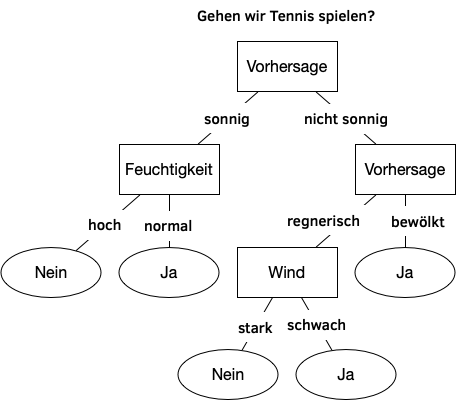
\includegraphics[width=9cm]{01-Abb_Entscheidungsbaum_Tennis.png}
\end{center}

\begin{aufgabe}
	Studieren sie die Dokumentation der Klasse \code{BinaryTree<ContentType>} und vergleichen sie sie mit der Verwendung der Klasse im Projekt \enquote{\emph{Entscheidungsbaum}} im Tauschordner (in der Klasse \code{Entscheider}).
	
	Versuchen sie die folgenden Leitfragen für sich zu beantworten:
	\begin{itemize}
		\item Wieso wird mehr als ein Objekt der Klasse \code{BinaryTree} erstellt?
		\item In welcher Reihenfolge wird der Baum aufgebaut (werden die Objekte der Knoten instanziiert)?
		\item Wie werden die Inhalte vom generischen Typ \code{ContentType} (hier Unterklassen der Klasse \code{Entschiedung}) im Baum gespeichert?
	\end{itemize}
\end{aufgabe}


\begin{aufgabe}
	Die Knoten enthalten Objekte der Unterklassen von \code{Entschiedung}. Jede Unterklasse entscheidet für einen Datensatz, ob es im Baum links oder rechts weiter geht. Die Blattknoten enthalten keine Entscheidung, sondern die finale Festlegung einer Klasse für den Datensatz (hier \enquote{Ja} oder \enquote{Nein}).
	
	Studieren sie die Klasse \code{Entscheidung} und ihre Unterklassen. Implementieren sie dann am Beispiel der Klasse \code{EntscheidungVorhersage1} eine Klasse \code{EntscheidungVorhersage2}, die die Entscheidung
	zwischen \enquote{regnerisch} und \enquote{bewölkt} umsetzt (vgl. Abbildung oben).
	
	Implementieren sie dann auch die anderen Unterklassen von \code{Entscheidung}.
\end{aufgabe}

\begin{aufgabe}
	Implementieren sie anhand des Beispiels im Konstruktor der Klasse \code{Entscheider} den vollständigen Entscheidungsbaum zur Tennis-Frage (vgl. Abbildung oben).
	
	Testen sie ihren Baum mit dem \emph{Objektinspektor} von BlueJ.
\end{aufgabe}

\begin{aufgabe}
	Vervollständigen sie die Methode \code{testeDatensatz} in Entscheider, so dass für einen Datensatz am Ende die korrekte Entscheidung (als \code{String}) zurückgegeben wird.
	
	Testen sie mit verschiedenen Datensätzen.
\end{aufgabe}

\end{document}
